\documentclass[11pt]{article}
\usepackage[utf8]{inputenc}
\usepackage{caption}
\usepackage{subcaption}
\usepackage{url}

\usepackage{ifpdf}
\ifpdf
\usepackage[pdftex]{graphicx}
\else
\usepackage{graphicx}
\fi

\usepackage[margin=1.15in]{geometry}


\title{6.830 Final Project Report \\ Hive Join Optimization}
\author{Kainar Kamalov, Maksim Stepanenko, Tiffany Lin}

\date{May 2012}

\begin{document}


\setlength{\baselineskip}{1.3\baselineskip}

\ifpdf
\DeclareGraphicsExtensions{.pdf, .jpg, .tif}
\else
\DeclareGraphicsExtensions{.eps, .jpg}
\fi

\maketitle

\section{Introduction}
Hive is a data warehouse infrastructure built on top of Hadoop for providing data for summarization, query, and analysis. In this project we tried two different approaches to optimizing Hive's join algorithm. The first approach is based on the estimated cost model computed during the runtime, and the second approach is based on the estimation of the hash table growth in order to make decisions. To see the benefit of our optimizations we compared the optimized system's performance with the original version using our constructed join-heavy queries and the data generated for TPC-H benchmark \cite{tpc-h}. In the remainder of this paper first we are going to discuss Hive's current join algorithm implementation and the relevant parts of its architecture. Next we will present and discuss the results of running TPC-H benchmark on Hive's original implementation. After that we will talk about the two methods we used to optimize the algorithm and the results they produced, we will also compare them to the results produced by the original implementation. We will conclude by summarizing our TPC-H benchmark, and the optimization results and by discussing if the optimizations we implemented were worthwhile for the given workloads.
\section{Hive Architecture and Join Algorithm}
In this section we will discuss the way join operations work in Hive and describe the architecture responsible for them. Hive is an infrastructure on top of Hadoop (an open-source implementation of Google's Map-Reduce framework); it compiles SQL queries into map-reduce jobs and runs them in a cluster. Since join is one of the most heavily used SQL operations and since often it is the bottleneck in the performance of query processing, we decided to look into optimizing it. Currently the join operation on Hive consists of two different options for executing a join operation: Common Join Task and Map Join Task. 
\subsection{Common Join Task}
\begin{figure}
	      \centering
                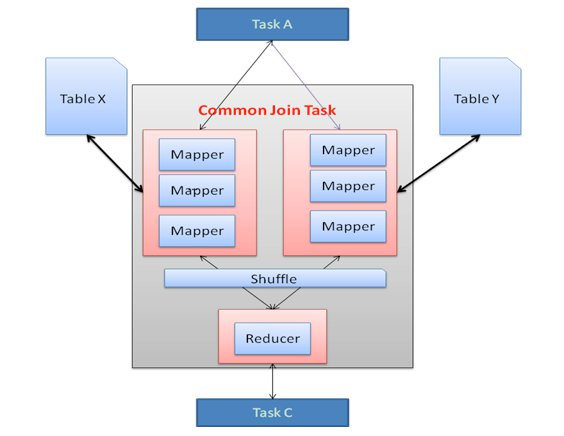
\includegraphics[scale=0.75]{common.jpg}
              \caption{Common Join Task \cite{facebook-join}}
              \label{fig:common-join}
\end{figure}

A common join task compiles into a regular map-reduce job with both map and reduce stages, as shown in Figure~\ref{fig:common-join}. In the map 

\subsection{Map Join Task}
Talk about Map join task here

\begin{figure}
	      \centering
                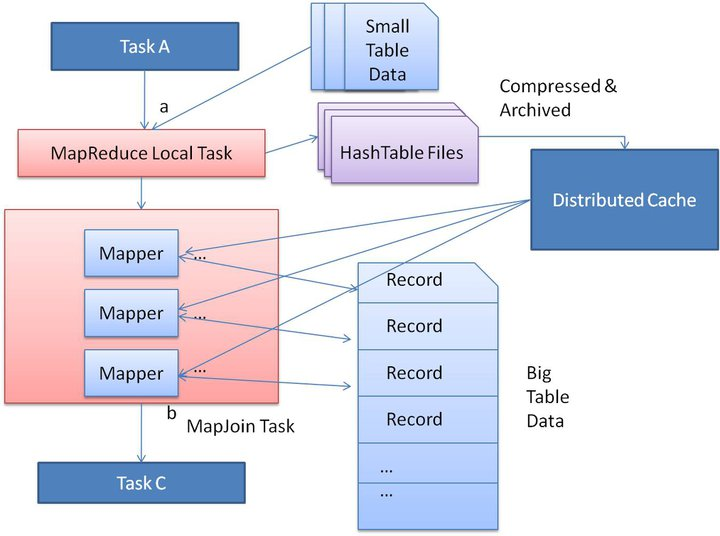
\includegraphics[scale=1]{mapjoin.jpg}
              \caption{Map Join Task \cite{facebook-join}}
              \label{fig:map-join}
\end{figure}

\section{Cost Model Estimation}

\section{Hive Hash Table Growth Estimation}

\section{TPC-H Benchmark Results}

\section{Discussion}
\section{Conclusion}

\bibliographystyle{plain}
% Stuff will show up here if you use BibTeX
\begin{thebibliography}{77}
\bibitem{tpc-h}
\url{http://www.tpc.org/tpch/}

\bibitem{facebook-join}
\author{Liyin Tang},
\url{https://www.facebook.com/note.php?note_id=470667928919}

\end{thebibliography}

\bibliography{}

\end{document}

